
\clearpage
\section{Customer Relationship Management}

Das CRM (Customer Relationship Management) ermöglicht Ihnen effizient Veranstaltungen (Anlässe, Präsentationen und Schulungen) zu koordinieren. Es unterstützt Sie bei der Einladung, dem Verwalten von Anmeldungen, Versenden von Erinnerungen und dem Erstellen von Teilnehmerlisten.

\vspace{\baselineskip}

Für Ihre Veranstaltung erstellen Sie über eine Webseite eine Einladung in Form eines Online-Flyers mit den wichtigsten Angaben zum Anlass, Eckdaten wie Termin, Zeit, Bemerkungen und Weiteres. Die Einladung, welche auf diese Einladungsseite verweist, versenden Sie aus dem CRM an eine gewünschte Personengruppe. Die Eingeladenen können über diese Webseite Ihre Anmeldung am Anlass durchführen (mittels Klick) oder falls notwendig zu Beginn oder später Ihre Entschuldigung einreichen. Sie als Organisator haben jederzeit den Überblick über die versendeten Einladungen und deren Status. Sie sehen sofort wie viele Personen sich bereits an- oder abgemeldet haben. \\

Schliesslich können Sie eine Teilnehmerliste exportieren und können auf diese Weise das Resultat Ihrer Einladung auswerten oder weiterreichen.

\vspace{\baselineskip}

Das CRM ist in zwei Teile gegliedert: 
\begin{itemize}
\item
\textbf{Veranstaltungstypen:} Hier legen Sie die verschiedenen Arten von Veranstaltungen fest (bspw. Jahresrückblick, Neuheiten-Präsentation etc.)
\item
\textbf{Veranstaltungen:} Unter diesem Menüpunkt werden die konkreten Veranstaltungen geplant. Nach dem Anlegen einer Veranstaltung haben Sie die Möglichkeit, die Einladungswebseite (Online-Flyer) zu gestalten.
\end{itemize}

\pagebreak
\subsection{Veranstaltungstypen}

\begin{wrapfigure}[7]{l}{6.5cm}   % [x] Wie manche Zeile soll sich um die Grafik "brechen"
  \vspace{-35pt}      % Grundwert war 20; mit 30 schön oben beim Text ausgerichtet
  \begin{center}
    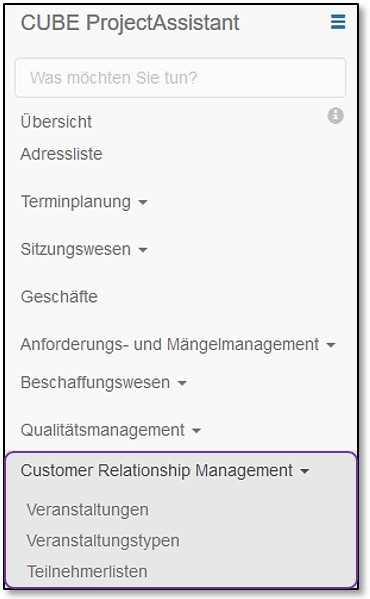
\includegraphics[width=1\linewidth]{../chapters/10_CRM/pictures/10-1-1_Menu_CRM.jpg}
  \end{center}
  \vspace{-20pt}
  \caption{Das CRM Menü}
  \vspace{-10pt}
\end{wrapfigure}

\textbf{Übersicht:} Klicken Sie im Menü links auf 'Customer Relationship Management' und den Unterpunkt Veranstaltungstypen.\\


\textbf{Hinweis:} Bevor Sie mit dem Erstellen einer Veranstaltung beginnen, erfassen Sie den oder die gewünschten Veranstaltungstyp/en. 

\vspace{8cm}

Die Übersicht der Veranstaltungstypen öffnet sich:

\begin{figure}[H]
\center{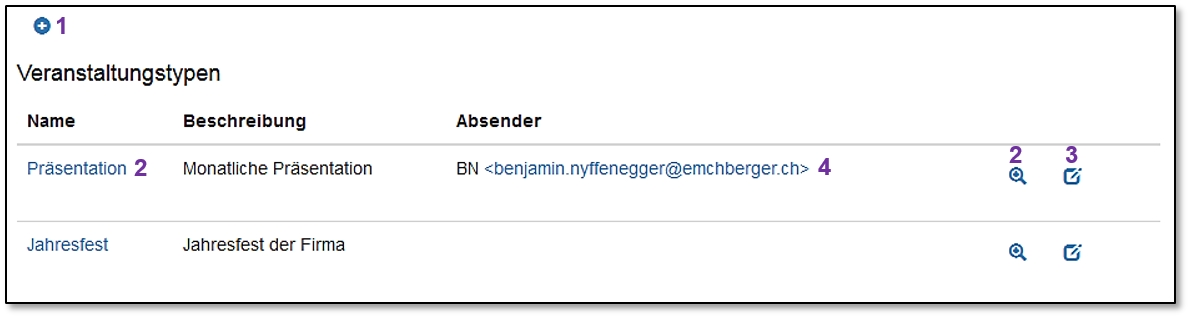
\includegraphics[width=1\linewidth]{../chapters/10_CRM/pictures/10-1_VeranstTyp_Uebersicht.jpg}}
\caption{Übersicht Veranstaltungstypen}
% \label{fig:speciation}
\end{figure}

Sie sehen alle erfassten Veranstaltungstypen. Mit Klick auf das Plussymbol 
\includegraphics[height=12pt]{/Icons/Plussymbol.jpg} \col{(1)} können Sie einen neuen Veranstaltungstyp erstellen. Mit Klick auf den entsprechenden Veranstaltungstyp \col{(2)} oder auf das Lupensymbol 
\includegraphics[height=12pt]{/Icons/Lupe.jpg} \col{(2)} können Sie die Details eines Veranstaltungstypen betrachten. Um einen Eintrag zu bearbeiten, klicken Sie auf das Bearbeiten-Symbol 
\includegraphics[height=12pt]{/Icons/Bearbeiten.jpg} \col{(3)}. Wurde eine Absender-Emailadresse hinterlegt, können Sie mit Klick auf diese \col{(4)} eine Email versenden. Wählen Sie das gewünschte Emailprogramm aus.

\subsubsection{Neue Veranstaltungstypen anlegen}

\begin{figure}[H]
\center{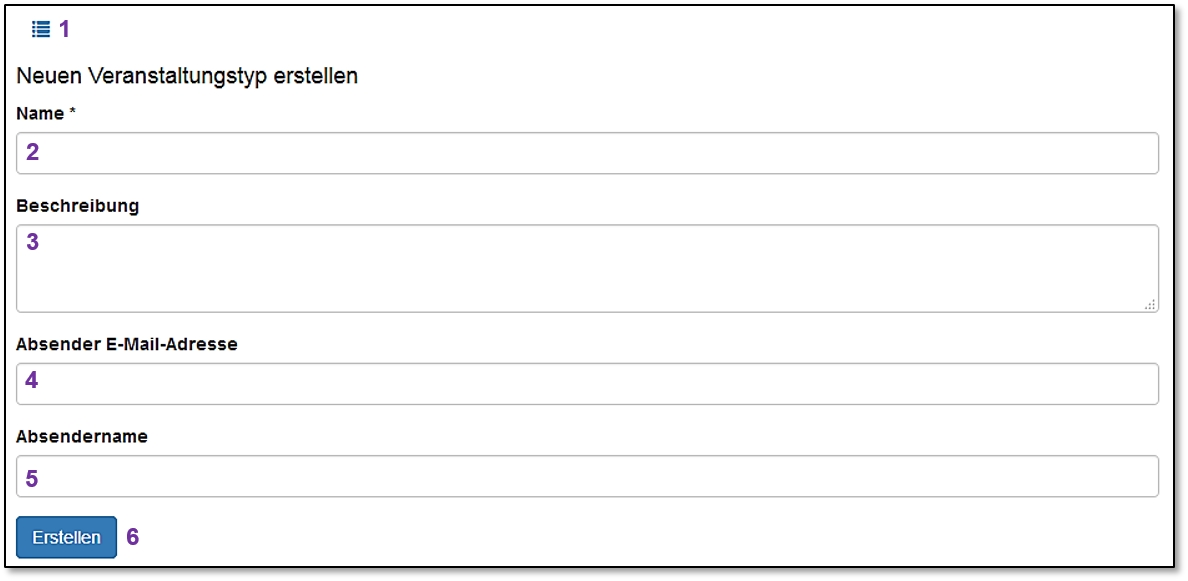
\includegraphics[width=1\linewidth]{../chapters/10_CRM/pictures/10-1_VeranstTyp_erstellen.jpg}}
\caption{Neue Veranstaltungstypen erstellen}
% \label{fig:speciation}
\end{figure}

Mit Klick auf das Listensymbol 
\includegraphics[height=12pt]{/Icons/Listensymbol_zurueck.jpg} \col{(1)} kehren Sie jederzeit auf die Übersicht zurück.\\
Geben Sie einen aussagekräftigen Namen \col{(2)} für den gewünschten Veranstaltungstyp ein (Dies ist ein Pflichtfeld und muss als einziges ausgefüllt werden.) Unter 'Beschreibung' \col {(3)} können Sie den Veranstaltungstyp präziser beschreiben. Sie haben die Möglichkeit eine Absender-Emailadresse \col{(4)} und einen Absendernamen \col{(5)} zu hinterlegen. Wird eine Emailadresse eingetragen, können Sie in der Übersicht mit Klick auf die Emailadresse direkt eine Email versenden. Nach den Eingaben schliessen Sie den Vorgang mit 'Erstellen' \col{(6)} ab.

\subsubsection{Bestehende Veranstaltungstypen betrachten und bearbeiten}

\begin{wrapfigure}[12]{l}{6.5cm}   % [x] Wie manche Zeile soll sich um die Grafik "brechen"
  \vspace{-35pt}      % Grundwert war 20; mit 30 schön oben beim Text ausgerichtet
  \begin{center}
    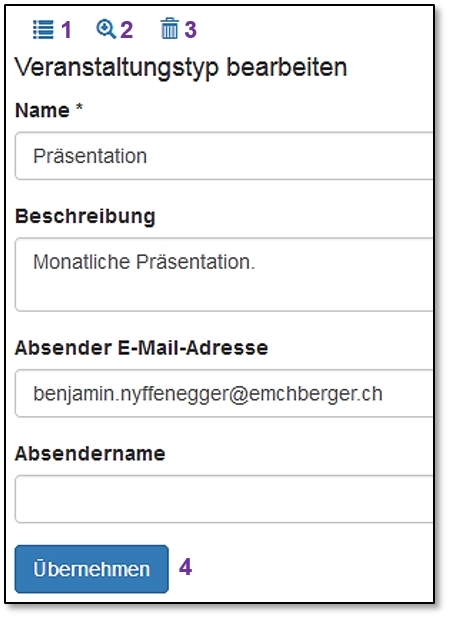
\includegraphics[width=1\linewidth]{../chapters/10_CRM/pictures/10-1-2_Veranstaltungstyp_bearbeiten.jpg}
  \end{center}
  \vspace{-20pt}
 % \caption{Veranstaltungstyp bearbeiten}
  \vspace{-10pt}
\end{wrapfigure}

Klicken Sie in der Übersicht der Veranstaltungstypen auf das Bearbeiten-Symbol 
\includegraphics[height=12pt]{/Icons/Bearbeiten.jpg}, um einen bereits erstellen Eintrag zu ändern. Die Maske mit den ausgefüllten Feldern wird geöffnet. Schliessen Sie diesen Vorgang mit Klick auf 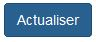
\includegraphics[height=12pt]{/Icons/B_Uebernehmen.jpg} \col{(4)} ab. Die Maske wird nicht automatisch geschlossen. Mit Klick auf das Listensymbol 
\includegraphics[height=12pt]{/Icons/Listensymbol_zurueck.jpg} \col{(1)} kehren Sie zur Übersicht zurück. Sie können mittels dem Lupensymbol 
\includegraphics[height=12pt]{/Icons/Lupe.jpg} \col{(2)} den Eintrag betrachten. Im Bearbeitungsmodus haben Sie zudem die Möglichkeit, mittels Klick auf das Mülltonnensymbol 
\includegraphics[height=12pt]{/Icons/Muelltonne.jpg} \col{(3)} einen Eintrag zu löschen.

\vspace{\baselineskip}

\subsection{Veranstaltungen}

Klicken Sie links im Menü unter 'Customer Relationship Management' den Unterpunkt Veranstaltungen. Sie erhalten die Übersicht über alle aufgenommen Veranstaltungen:

\begin{figure}[H]
\center{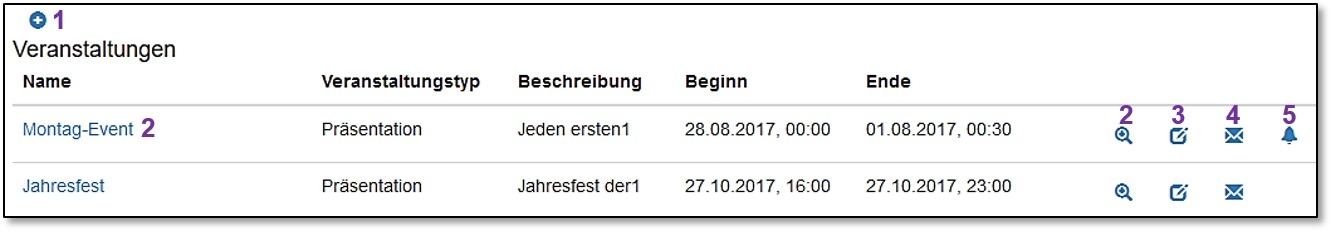
\includegraphics[width=1\linewidth]{../chapters/10_CRM/pictures/10-2_Veranstaltungen_Uebersicht.jpg}}
\caption{Übersicht Veranstaltungen}
% \label{fig:speciation}
\end{figure}

Mit Klick auf das Plussymbol 
\includegraphics[height=12pt]{/Icons/Plussymbol.jpg} \col{(1)} können Sie neue Veranstaltungen hinzufügen. Wenn Sie auf den blauen Veranstaltungstitel oder das Lupensymbol 
\includegraphics[height=12pt]{/Icons/Lupe.jpg} \col{(2)} klicken, können Sie einen Eintrag anschauen. Um eine Veranstaltung zu bearbeiten, klicken Sie auf das Bearbeiten-Symbol 
\includegraphics[height=12pt]{/Icons/Bearbeiten.jpg} \col{(3)}. Mit Klick auf das Mailsymbol 
\includegraphics[height=12pt]{/Icons/Briefsymbol.jpg} \col{(4)} gelangen Sie in den Versandmodus, in welchem Sie die Email-Vorlage bearbeiten können.

\subsubsection{Neue Veranstaltungen anlegen}

Klicken Sie auf das Plussymbol 
\includegraphics[height=12pt]{/Icons/Plussymbol.jpg} in der Veranstaltungsübersicht, um eine neue Veranstaltung anzulegen.

\begin{wrapfigure}[15]{l}{6.5cm}   % [x] Wie manche Zeile soll sich um die Grafik "brechen"
  \vspace{-25pt}      % Grundwert war 20; mit 30 schön oben beim Text ausgerichtet
  \begin{center}
    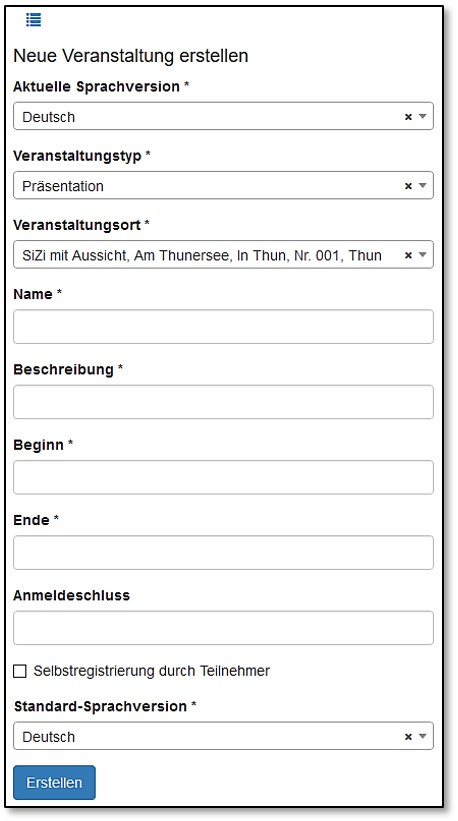
\includegraphics[width=1\linewidth]{../chapters/10_CRM/pictures/10-2-1_NeueVeranstaltung.jpg}
  \end{center}
  \vspace{-20pt}
  % \caption{Neue Veranstaltung anlegen}
  \vspace{-10pt}
\end{wrapfigure}

Die Eingabemaske erscheint. Bei den Feldern 'Veranstaltungstyp' und 'Veranstaltungsort' handelt es sich um Dropdown-Listen. Wählen Sie unter den Einträgen den gewünschten aus.\\
\textbf{Hinweis:} Die Veranstaltungsorte müssen vorgängig durch einen Administrator oder berechtigten CUBE PA Superuser in der Konfiguration hinterlegt werden. Bei Fragen können Sie eine Email an den CUBE PA Support senden: {\color{red} cube.support@emchberger.ch}.\\
Die meisten Felder sind Pflichtfelder und müssen ausgefüllt werden. Sind alle Eingaben gemacht klicken Sie auf den 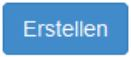
\includegraphics[height=12pt]{/Icons/B_Erstellen.jpg}-Button. Die Veranstaltung wird gespeichert und weitere Optionen werden nun angezeigt:

\begin{figure}[H]
\center{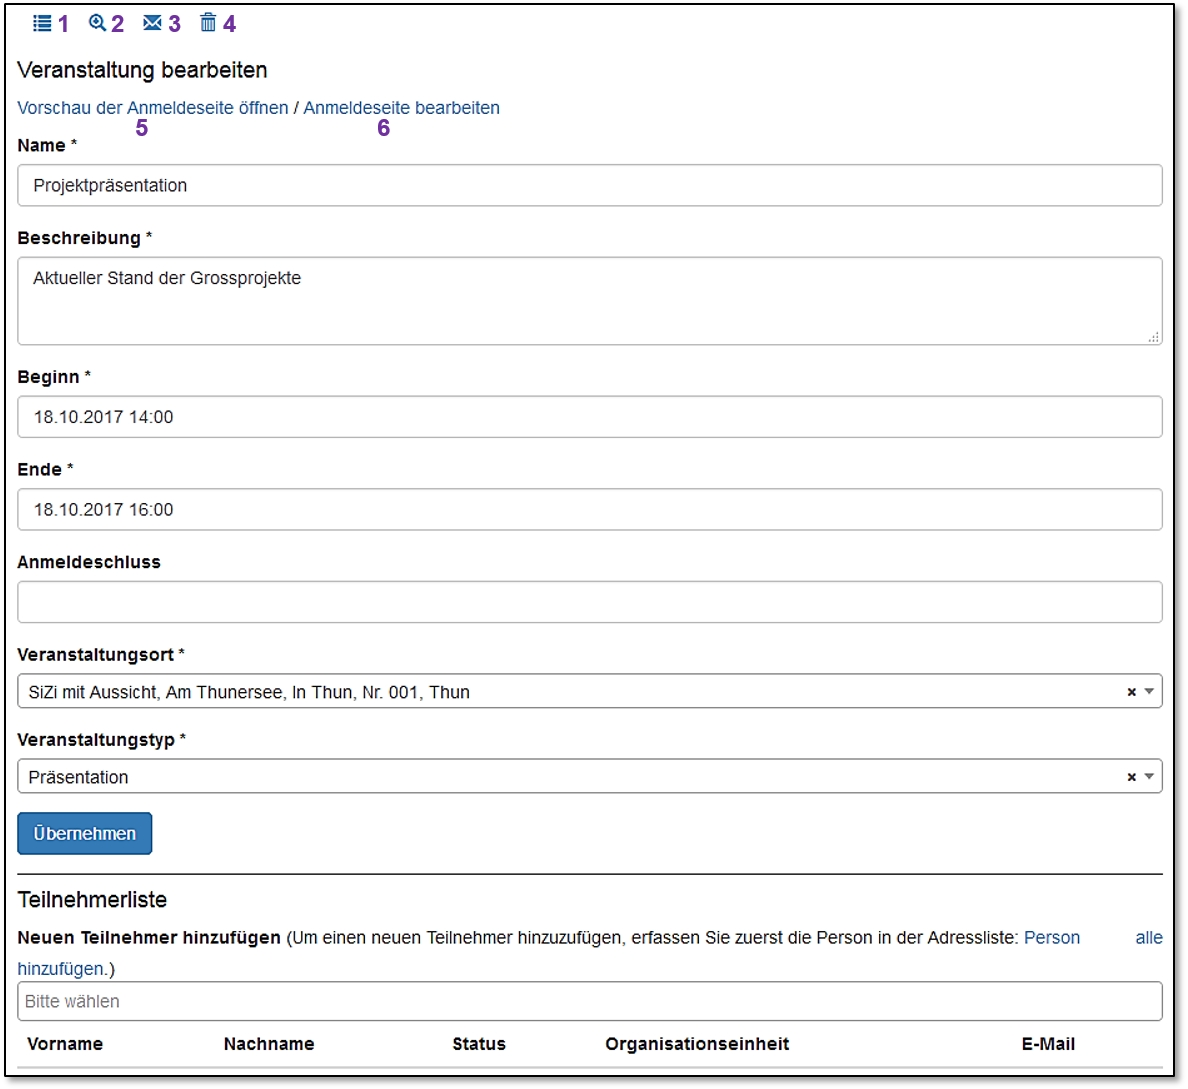
\includegraphics[width=1\linewidth]{../chapters/10_CRM/pictures/10-2-1_NeueVeranstaltung_erweitert.jpg}}
\caption{Neue Veranstaltung anlegen - erweiterte Ansicht}
% \label{fig:speciation}
\end{figure}

Im unteren Bereich der Eingabemaske wird die Teilnehmerliste eingeblendet. Mehr über die Teilnehmerliste finden Sie im nächsten Kapitel \ref{bkm:Ref112017102}. Kehren Sie mit Klick auf das Listensymbol 
\includegraphics[height=12pt]{/Icons/Listensymbol.jpg} \col{(1)} zur Veranstaltungsübersicht zurück. Verlassen Sie den Bearbeitungsmodus mit Klick auf die Lupe 
\includegraphics[height=12pt]{/Icons/Lupe.jpg} \col{(2)} oder wechseln Sie in die Mailvorlagenansicht mittels dem Mailsymbol 
\includegraphics[height=12pt]{/Icons/Briefsymbol.jpg} \col{(3)}. Sie haben auch die Möglichkeit eine Veranstaltung zu löschen. Dazu klicken Sie auf das Mülltonnensymbol 
\includegraphics[height=12pt]{/Icons/Muelltonne.jpg} \col{(4)}.\\
Nun haben Sie auch die Möglichkeit die Einladungsseite (Online-Flyer) zu erstellen. Mit Klick auf den blauen Text 'Anmeldeseite bearbeiten' \col{(6)} gelangen Sie auf die Gestaltungswebseite. Mit Klick auf den blauen Text 'Vorschau der Anmeldeseite öffnen' \col{(5)} können Sie Ihre Einladungsseite ansehen. Mehr dazu im Kapitel \ref{bkm:Ref112017101} (Einladungsseite gestalten).

\subsubsection{Teilnehmer verwalten}
\label{bkm:Ref112017102}

\textbf{Hinweis:} Vorgängig müssen Teilnehmer in der Adressliste erfasst werden, damit sie im CRM zur Auswahl zur Verfügung stehen. Sie haben jedoch die Möglichkeit, von der Teilnehmerverwaltung des CRM mit einem Klick direkt in die Adressliste zu wechseln \col{(1)}, um neue Teilnehmer zu erfassen. Mehr zum Thema Personen und Firmen in der Adressliste erfassen, finden Sie im Kapitel \ref{bkm:Ref443738751}.

\vspace{\baselineskip}

\textbf{Hinweis zum Speichern beim Hinzufügen von Teilnehmern:} Werden Teilnehmer ausgewählt, wird diese Auswahl gerade gespeichert. Deshalb ist die Funktion 'alle' Teilnehmer \col{(2)} (alle Personen aus der Adressliste) hinzuzufügen nur mit Vorsicht anzuwenden. Mit einem Klick haben Sie ihre ganze Adressliste in der Einladung gespeichert.

\vspace{\baselineskip}

Mit Klick auf 'alle' \col{(2)} werden sämtliche Personen in der Adressliste einer Einladung hinzugefügt. Beachten Sie obigen Hinweis zum Speichern. Sie können die Personen mit Vor- oder Nachnamen direkt in das Suchfeld \col{(3)} eintragen und aus des gefunden Einträgen mit Mausklick auswählen. Die Suche funktioniert auch mit Eingabe von Firmennamen; sämtliche Personen einer gesuchten Firma werden angezeigt. \\
Wurden Teilnehmer ausgewählt, wird der Status automatisch auf 'neu' gesetzt. Dieser lässt sich mit dem Stiftsymbol 
\includegraphics[height=12pt]{/Icons/Stift.jpg} \col{(4)} ändern. Mit Klick auf das Kreuzsymbol 
\includegraphics[height=12pt]{/Icons/Kreuzchen.jpg} \col{(5)} können Teilnehmer wieder gelöscht werden. Da sämtliche Mutationen gerade gespeichert werden, müssen Sie nicht auf 'Übernehmen' klicken.

\begin{figure}[H]
\center{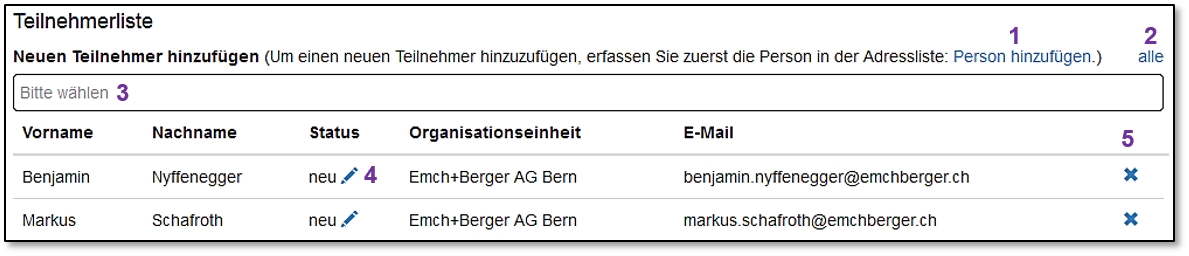
\includegraphics[width=1\linewidth]{../chapters/10_CRM/pictures/10-2-2_Teilnehmerliste.jpg}}
\caption{Teilnehmerliste bearbeiten}
% \label{fig:speciation}
\end{figure}

\textbf{Teilnehmerlsiten exportieren}

Im Betrachtungsmodus 
\includegraphics[height=12pt]{/Icons/Lupe.jpg} haben Sie die Möglichkeit mit Klick auf das Downloadsymbol 
\includegraphics[height=12pt]{/Icons/Download.jpg} \col{(1)} eine Teilnehmerlsite im Excel (.xlsx) zu exportieren.

\begin{figure}[H]
\center{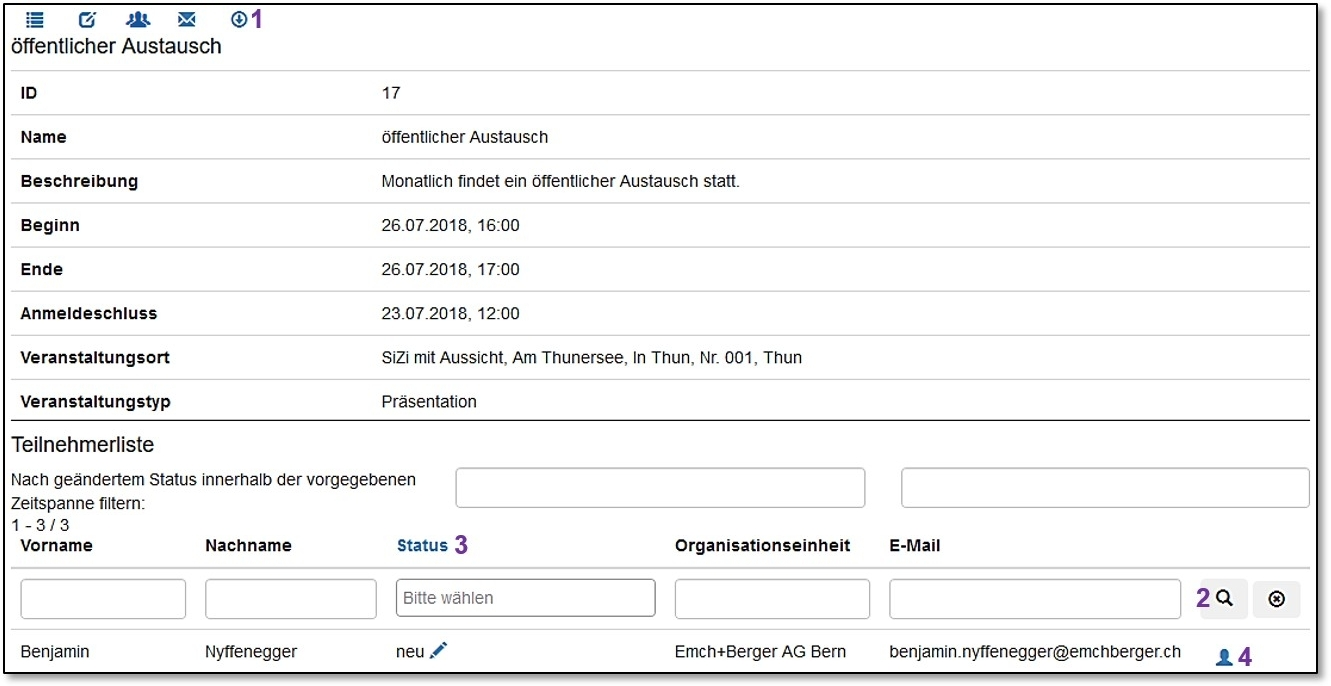
\includegraphics[width=.7\linewidth]{../chapters/10_CRM/pictures/10-2-2_Teilnehmerliste_exportieren.jpg}}
\caption{Teilnehmerliste exportieren}
% \label{fig:speciation}
\end{figure}

Ebenso können Sie im Betrachtungsmodus 
\includegraphics[height=12pt]{/Icons/Lupe.jpg} in der Teilnehmerliste nach den verschiedenen Feldern (Vorname, Nachnamen, Status, Organisationseinheit und Email) suchen und die Einträge nach dem Status sortieren. Mit Klick auf das Personensymbol  
\includegraphics[height=12pt]{/Icons/Person.jpg} können Sie direkt in der Adressliste den Eintrag einer Person ändern. Um von der Adressliste wieder zum CRM zurückzukehren, schliessen Sie nach dem Speichern (Klick auf 'Übernehmen') das zusätzlich geöffnete Browserfenster.

\subsubsection{Einladungsseite gestalten (Online-Flyer)}
\label{bkm:Ref112017101}

Klicken Sie im Bearbeitungsmodus der Einladung auf den blauen Text 'Anmeldeseite bearbeiten' \col{(5)}. 

\begin{figure}[H]
\center{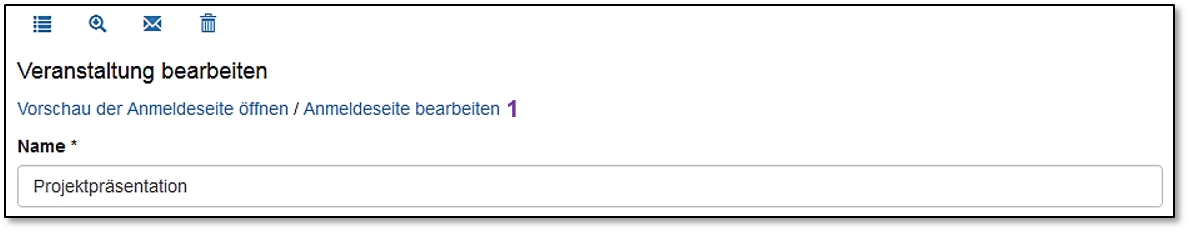
\includegraphics[width=1\linewidth]{../chapters/10_CRM/pictures/10-2-3_Einladung_gestalten_Link.jpg}}
\caption{Einladungsseite gestalten}
% \label{fig:speciation}
\end{figure}

Nun wird eine leere Editierseite der Onlineeinladung geöffnet:

\begin{figure}[H]
\center{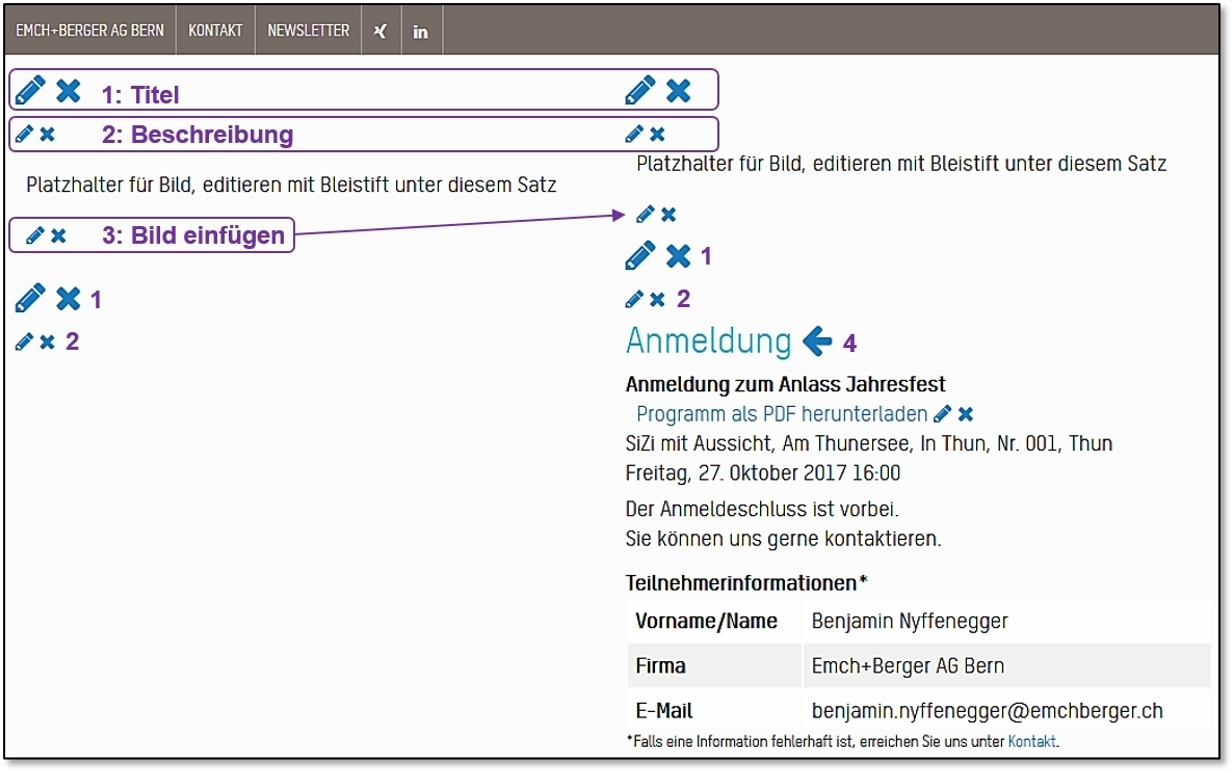
\includegraphics[width=1\linewidth]{../chapters/10_CRM/pictures/10-2-3_Leere_Einladung.jpg}}
\caption{Leere Einladungsseite}
% \label{fig:speciation}
\end{figure}

Mit dem Stiftsymbol 
\includegraphics[height=12pt]{/Icons/Stift.jpg} können Sie nun die verschiedenen Bereiche gestalten. Mit dem Kreuzsymbol 
\includegraphics[height=12pt]{/Icons/Kreuzchen.jpg} können Sie Bereiche löschen.
Die grossen Icons stehen für einen Titel \col{(1)}. Mit Klick auf den Stift 
\includegraphics[height=12pt]{/Icons/Stift.jpg} öffnet sich ein reines Textfeld, in welchem Sie den Titel des Bereiches eingeben und mit dem Gutzeichen 
\includegraphics[height=12pt]{/Icons/Gutzeichen.jpg} speichern können.
Mit Klick auf den Stift 
\includegraphics[height=12pt]{/Icons/Stift.jpg} für die Beschreibung \col{(2)} öffnet sich ein ausführliches Editierfenster, in welchem Sie den Text nach Belieben formatieren können (siehe unten). Unterhalb des Textes 'Platzhalter für Bild, editieren mit Bleistift unter diesem Satz' können Sie mit Klick auf den Stift 
\includegraphics[height=12pt]{/Icons/Stift.jpg} ein Bild hochladen, indem Sie auf 'Durchsuchen' klicken und das gewünschte Bild auswählen und mit dem Gutzeichen 
\includegraphics[height=12pt]{/Icons/Gutzeichen.jpg} bestätigen. 

\begin{figure}[H]
\center{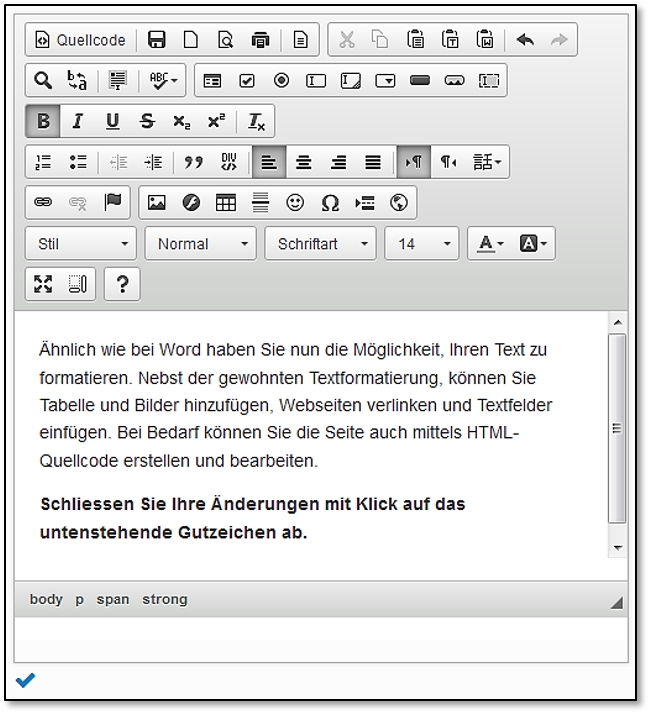
\includegraphics[width=.7\linewidth]{../chapters/10_CRM/pictures/10-2-3_Text_formatieren.jpg}}
\caption{Text formatieren}
% \label{fig:speciation}
\end{figure}


% \subsubsection{Einladungen versenden}

% inkl. Emailvorlage bearbeiten

% \subsubsection{Bestehende Veranstaltungen betrachten und bearbeiten}

% Veranstaltung löschen
% Text x

